%%%%%%%%%%%%%%%%%%%%%%%%%%%%%%%%%%%%%%%%%
% Beamer Presentation
% LaTeX Template
% Version 1.0 (10/11/12)
%
% This template has been downloaded from:
% http://www.LaTeXTemplates.com
%
% License:
% CC BY-NC-SA 3.0 (http://creativecommons.org/licenses/by-nc-sa/3.0/)
%
%%%%%%%%%%%%%%%%%%%%%%%%%%%%%%%%%%%%%%%%%

%----------------------------------------------------------------------------------------
%	PACKAGES AND THEMES
%----------------------------------------------------------------------------------------

\documentclass{beamer} 


\mode<presentation> {

% The Beamer class comes with a number of default slide themes
% which change the colors and layouts of slides. Below this is a list
% of all the themes, uncomment each in turn to see what they look like.

%\usetheme{default}
%\usetheme{AnnArbor}
%\usetheme{Antibes}
%\usetheme{Bergen}
%\usetheme{Berkeley}
%\usetheme{Berlin}
%\usetheme{Boadilla}
\usetheme{CambridgeUS}
%\usetheme{Copenhagen}
%\usetheme{Darmstadt}
%\usetheme{Dresden}
%\usetheme{Frankfurt}
%\usetheme{Goettingen}
%\usetheme{Hannover}
%\usetheme{Ilmenau}
%\usetheme{JuanLesPins}
%\usetheme{Luebeck}
%\usetheme{Madrid}
%\usetheme{Malmoe}
%\usetheme{Marburg}
%\usetheme{Montpellier}
%\usetheme{PaloAlto}
%\usetheme{Pittsburgh}
%\usetheme{Rochester}
%\usetheme{Singapore}
%\usetheme{Szeged}
%\usetheme{Warsaw}

% As well as themes, the Beamer class has a number of color themes
% for any slide theme. Uncomment each of these in turn to see how it
% changes the colors of your current slide theme.

%\usecolortheme{albatross}
\usecolortheme{beaver}
%\usecolortheme{beetle}
%\usecolortheme{crane}
%\usecolortheme{dolphin}
%\usecolortheme{dove}
%\usecolortheme{fly}
%\usecolortheme{lily}
%\usecolortheme{orchid}
%\usecolortheme{rose}
%\usecolortheme{seagull}
%\usecolortheme{seahorse}
%\usecolortheme{whale}
%\usecolortheme{wolverine}

%\setbeamertemplate{footline} % To remove the footer line in all slides uncomment this line
%\setbeamertemplate{footline}[page number] % To replace the footer line in all slides with a simple slide count uncomment this line

%\setbeamertemplate{navigation symbols}{} % To remove the navigation symbols from the bottom of all slides uncomment this line
}
\usepackage{amsmath} 
\usepackage{graphicx} % Allows including images
\usepackage{booktabs} % Allows the use of \toprule, \midrule and \bottomrule in tables


\DeclareMathOperator*{\argmax}{argmax} 
%\DeclareMathOperator*{\min}{min} 

%----------------------------------------------------------------------------------------
%	TITLE PAGE
%----------------------------------------------------------------------------------------

\title[]{Poisson Image Editing} % The short title appears at the bottom of every slide, the full title is only on the title page

\author{Jack Breeding, Ehasn Ahmai, Sek Cheong} % Your name
\institute[UW] % Your institution as it will appear on the bottom of every slide, may be shorthand to save space
{
University of Wisconsin, Madison \\ % Your institution for the title page
\medskip
\textit{\{jbreeding,eahmadi2, sucheong\}@wisc.com} % Your email address
}
\date{\today} % Date, can be changed to a custom date

\begin{document}

\begin{frame}
\titlepage % Print the title page as the first slide
\end{frame}

\begin{frame}
% Table of contents slide, comment this block out to remove it    
\frametitle{Overview} 
% Throughout your presentation, if you choose to use \section{} and \subsection{} commands, 
%these will automatically be printed on this slide as an overview of your presentation
\tableofcontents 
\end{frame}

%----------------------------------------------------------------------------------------
%	PRESENTATION SLIDES
%----------------------------------------------------------------------------------------


%------------------------------------------------
% Sections can be created in order to organize your presentation into discrete blocks, all sections and subsections 
% are automatically printed in the table of contents as an overview of the talk
\section{Motivation} 
%------------------------------------------------

% A subsection can be created just before a set of slides with a common theme to further break down your presentation into chunks
\subsection{Make local changes during image editing can be difficult}
\subsection{Traditional methods take a lot of time and leave noticeable seams}
\subsection{Laplacian pyramid approach can blend the edges but have color mismatch}

\begin{frame}
\frametitle{Motivation} 
    \begin{itemize}
        \item Make local changes during image editing can be difficult
        \item Traditional methods take a lot of time and leave noticeable seams
        \item Laplacian pyramid approach can blend the edges but have color mismatch 
    \end{itemize}
    \begin{figure}[!ht]
        \centering
        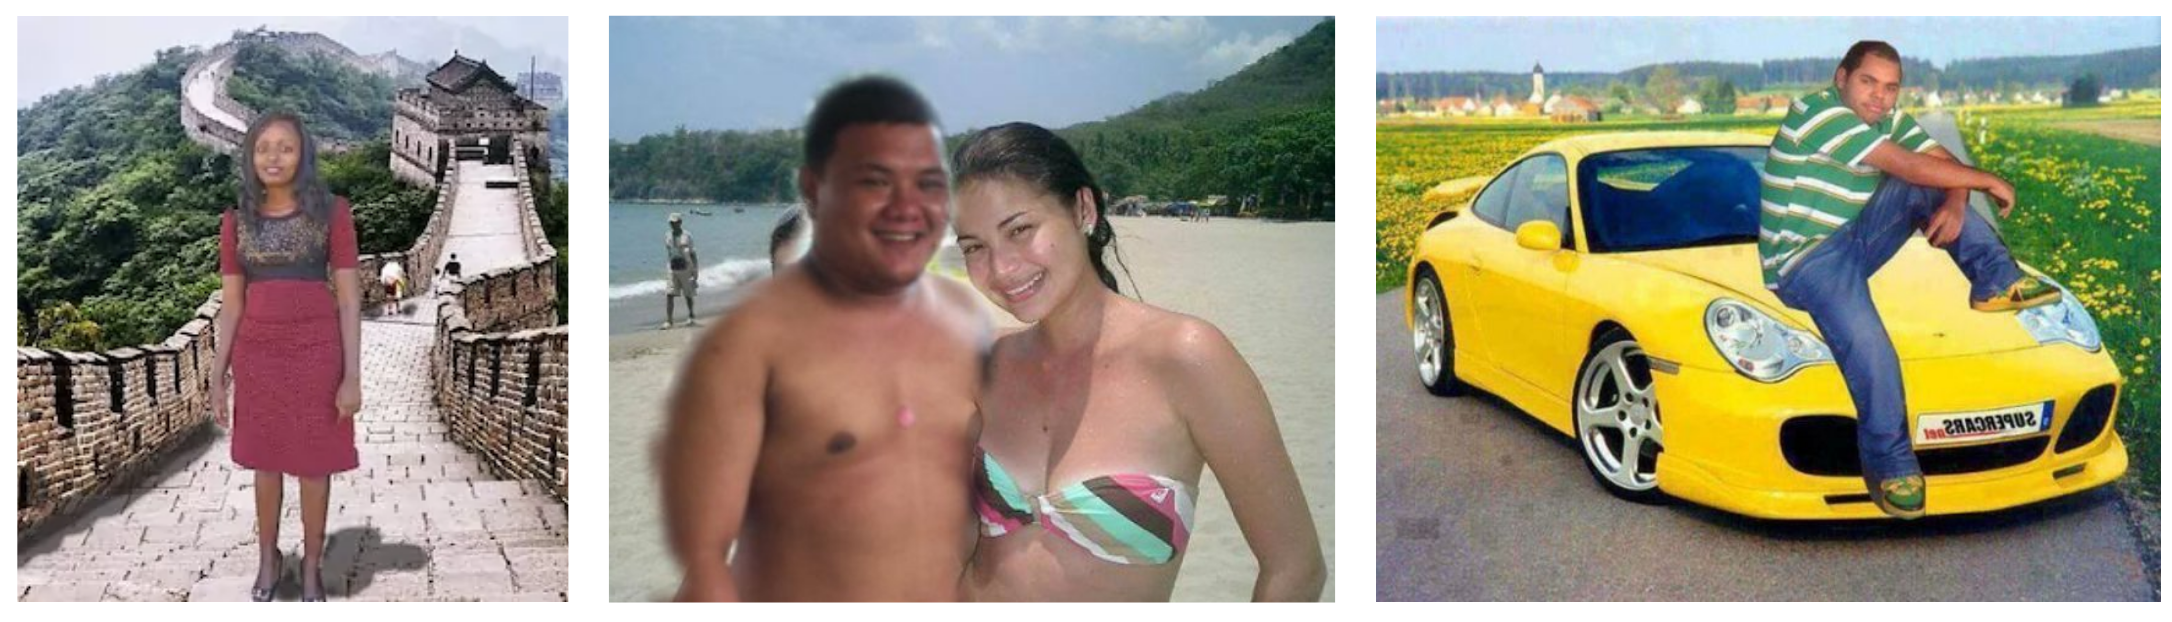
\includegraphics[width=2.8in]{resource/traditional.png}        
    \end{figure}
\end{frame}


\section{Approach} 
\begin{frame}
\subsection{Change in gradient domain} 
\subsection{Reconstruct image from gradient} 
\frametitle{Approach} 
    \begin{itemize}
        \item Change in gradient domain
        \item Reconstruct image from gradient        
    \end{itemize}
\end{frame}


% We will start by giving some basic definitions which will be used in the matematical constructs on 
% how possion editing works
\section{Mathematical Background} 
\subsection{Definition} 
\begin{frame}
\frametitle{Definition} 
    \begin{figure}[!ht]
        \centering
        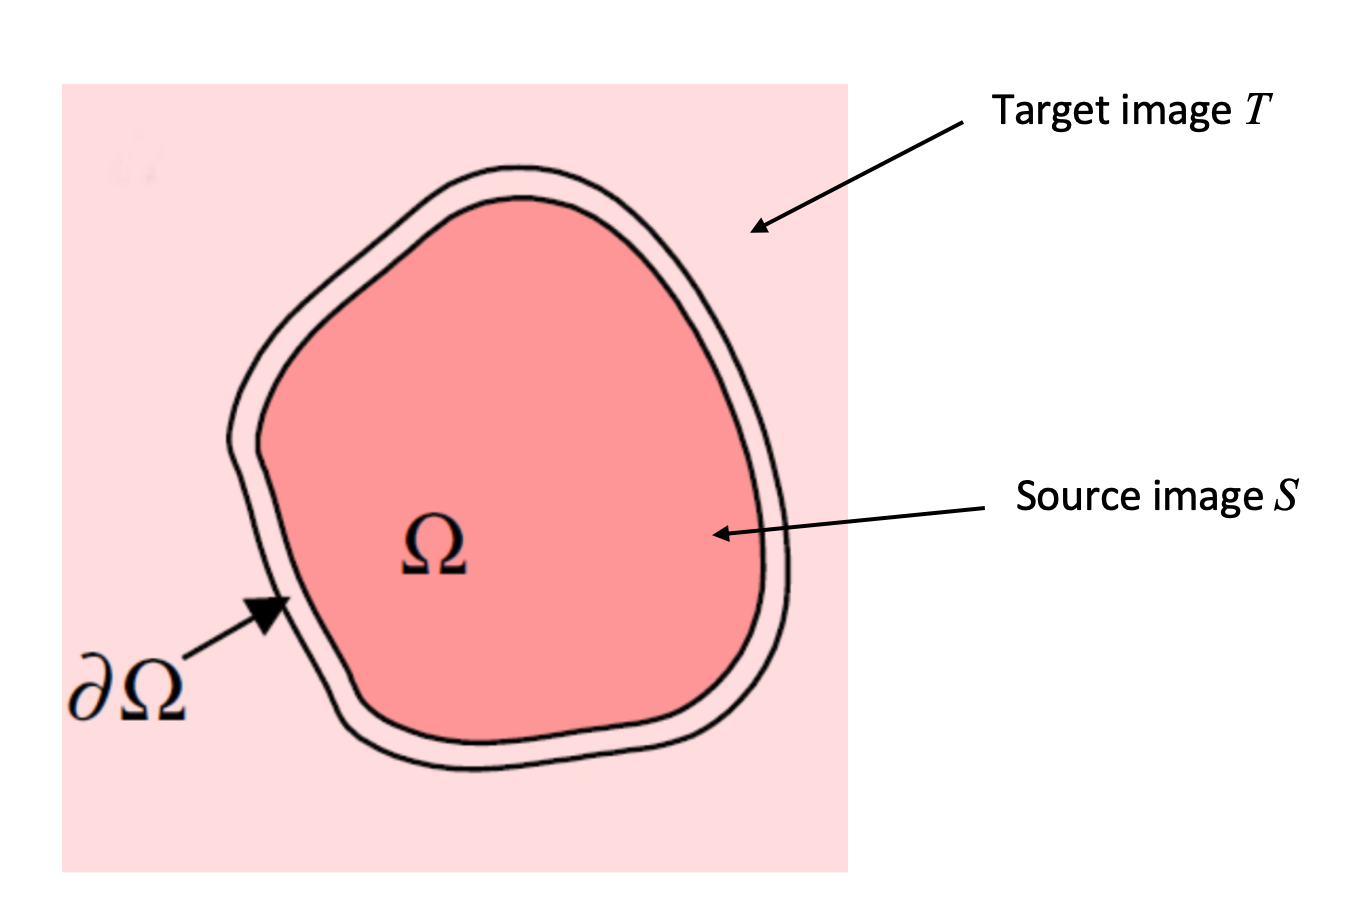
\includegraphics[width=2.8in]{resource/region.png}
    \end{figure}
    \begin{itemize}
        \item The source image $S(x,y)$ defined over a closed region $\Omega$
        \item The boundary of this region denoted as $\partial \Omega$
        \item The target image $T(x,y)$ defined some rectangular region in $\mathbb{R}^2$        
    \end{itemize}    
    % \begin{equation}
    %     \nabla (fg)= f\nabla g + g \nabla f
    % \end{equation}
\end{frame}

% Here we talk about the basic ideas behind possion image editing 
\subsection{Basic Idea} 

\begin{frame}
\frametitle{Basic Idea}
\begin{itemize}   
    \item Want to construct the composite image, $I(x,y)$, which should agree with $T(x,y)$ and look like $S(x,y)$    
    \item $I(x,y)$ should exactly agree with $T(x,y)$ 
    \item $I(x,y)$ ``look like'' $S(x,y)$ inside $\Omega$
    \item If we place directly $S$ over $T$ and smooth over the edges, the result maybe unacceptable, due to color mismatch
    \end{itemize}
\end{frame}

% The example of target and source images from the paper
\begin{frame}
\frametitle{Basic Idea}
\begin{figure}[!ht]
    \centering
    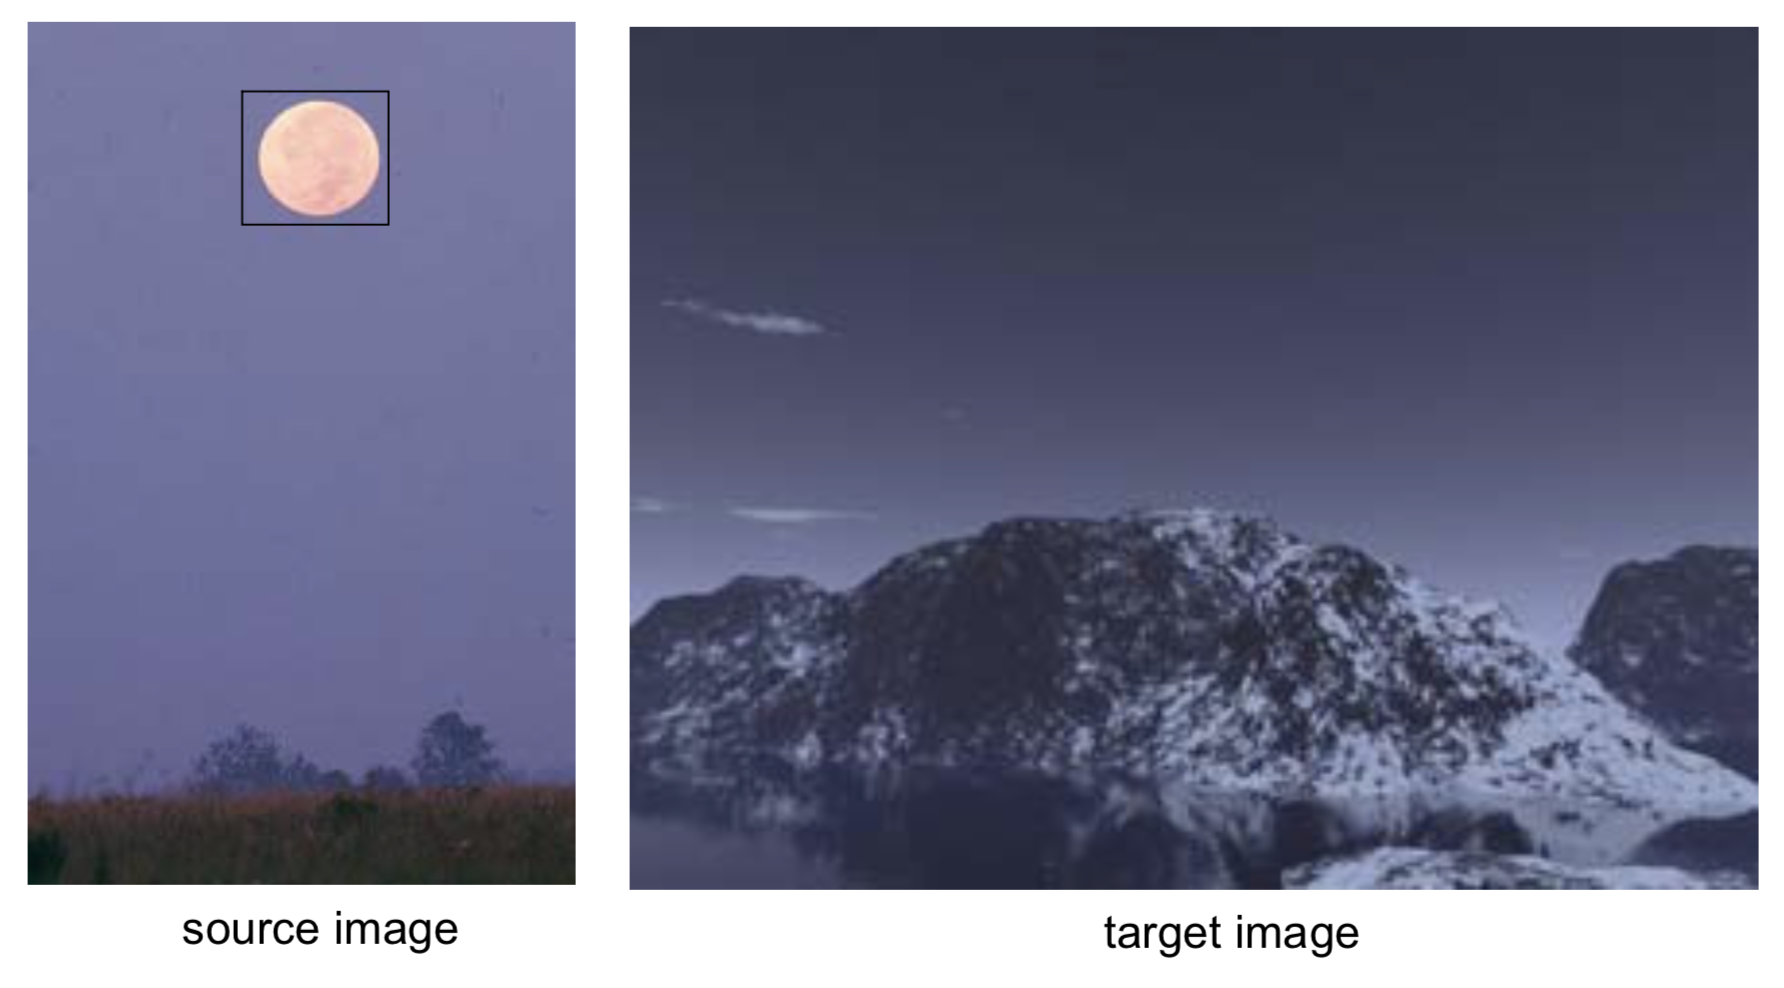
\includegraphics[width=3.8in]{resource/source_target_1.png}            
\end{figure}
\end{frame}

% The simple cloning, directly paste the source over the target results in ugly edges and mismatched color
% Laplacian pyramid based, multiresolution blending method, blends the edge but still results in interior 
% color mismatch
\begin{frame}
\frametitle{Basic Idea}
\begin{figure}[!ht]
    \centering
    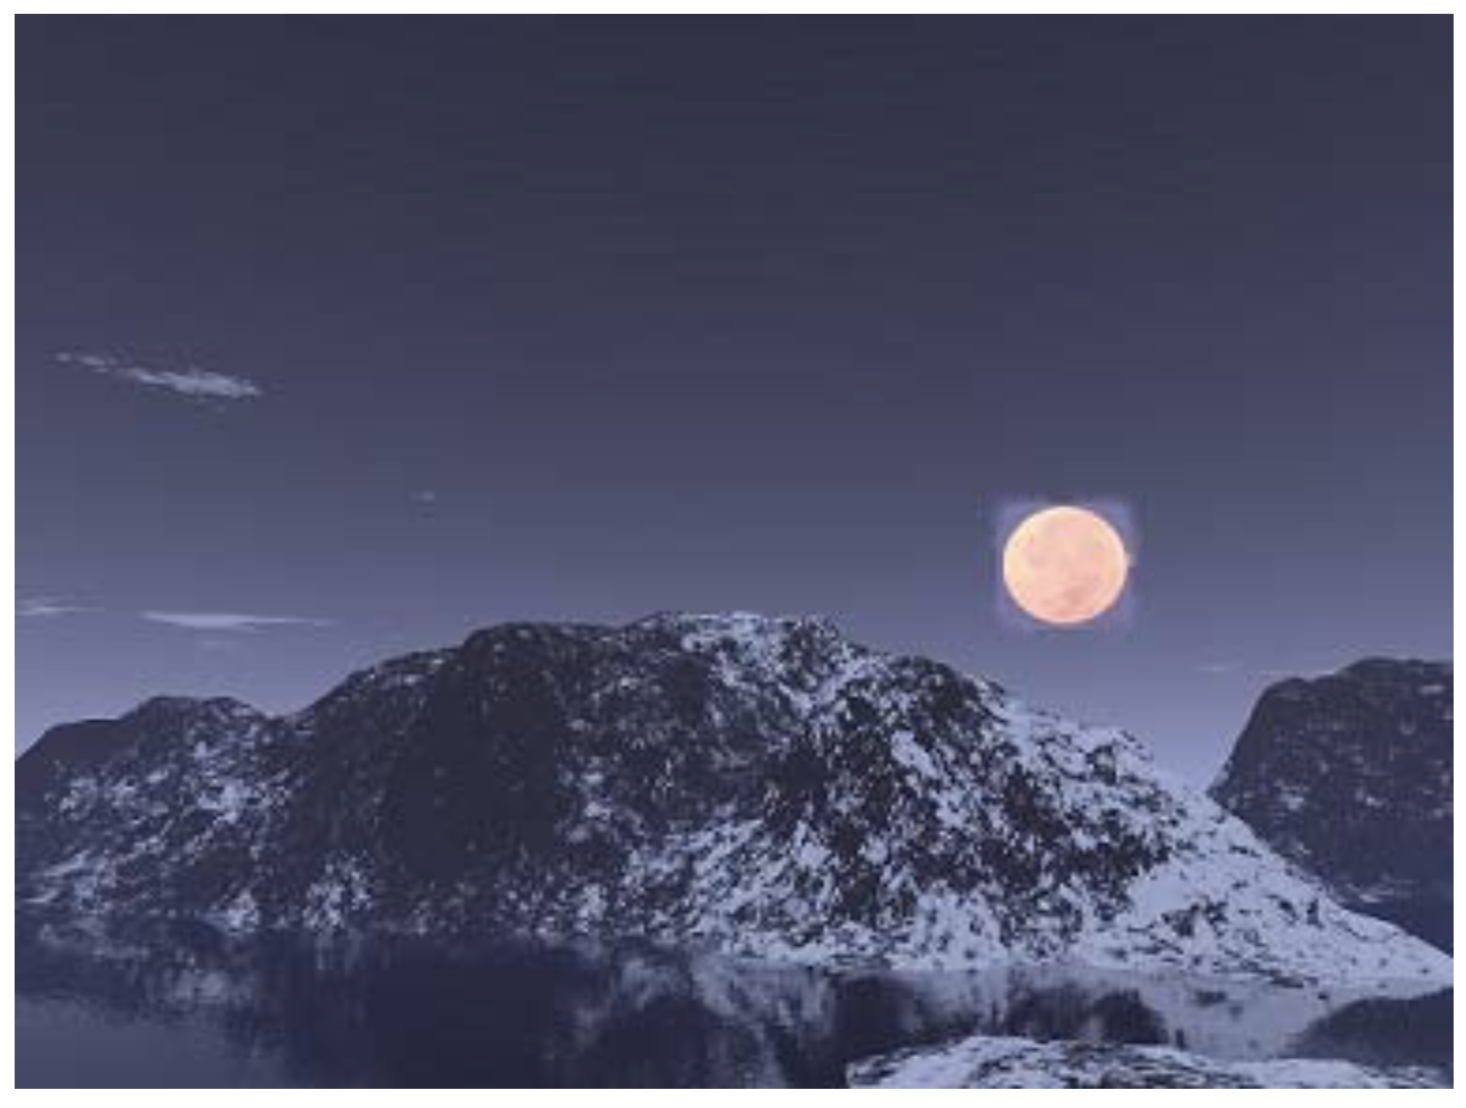
\includegraphics[width=3.0in]{resource/simple_cloning_1.png}        
    \caption{Simple cloning, background of source does not agree with the target}
\end{figure}
\end{frame}

\begin{frame}
\frametitle{Basic Idea}
\begin{figure}[!ht]
    \centering
    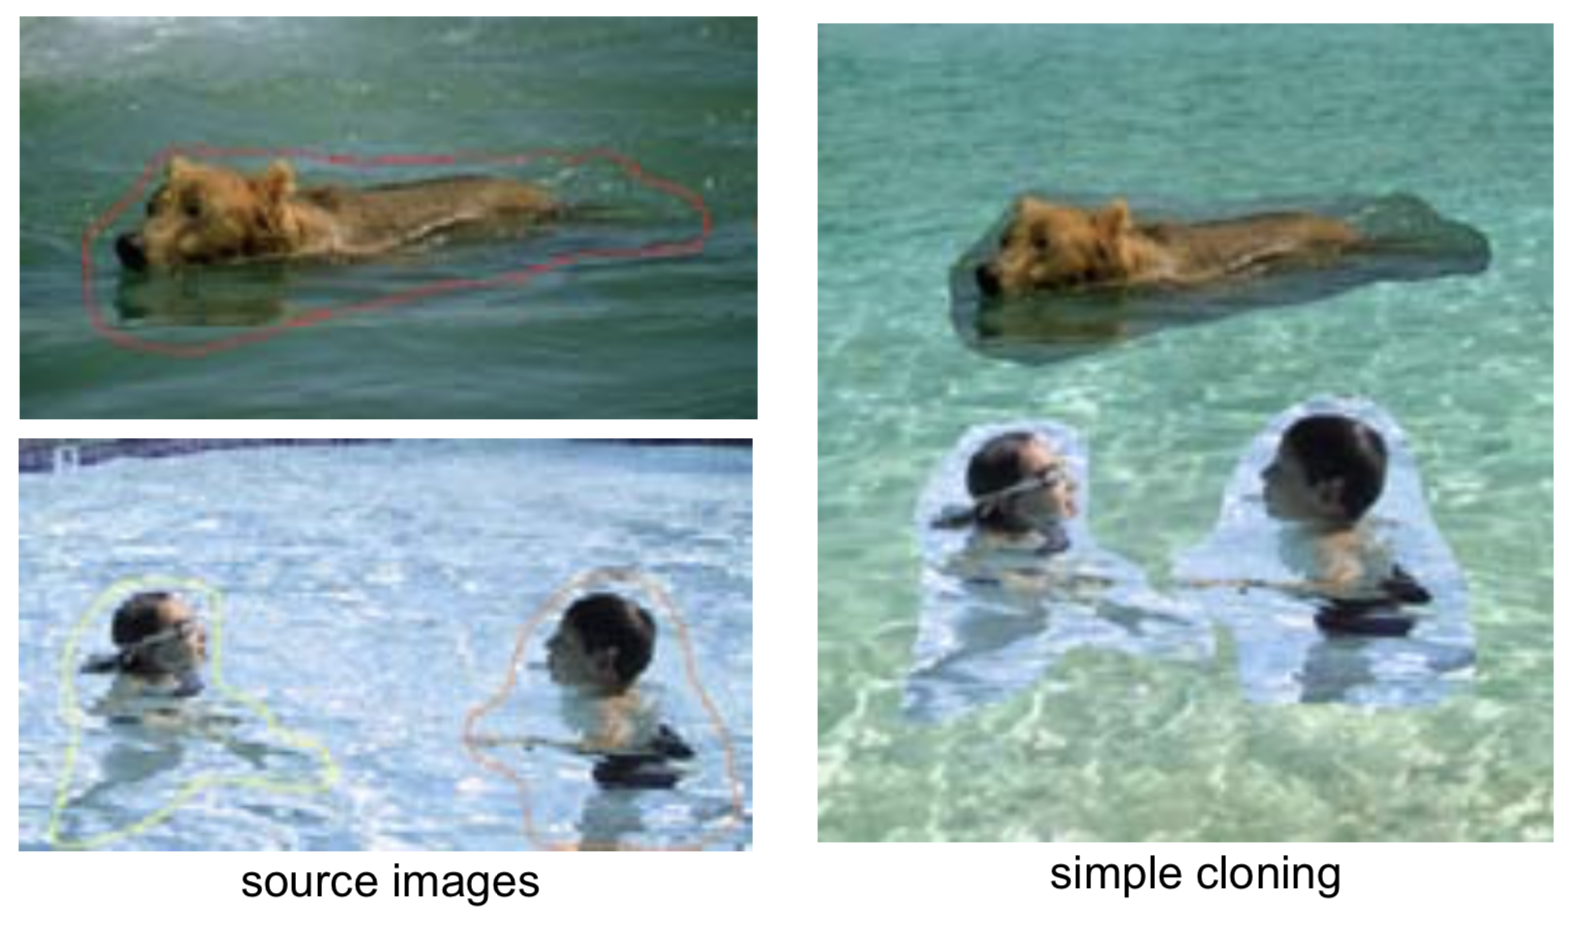
\includegraphics[width=3.8in]{resource/simple_cloning_2.png}        
\end{figure}
\end{frame}

\begin{frame}
    \frametitle{Basic Idea}
    \begin{figure}[!ht]
        \centering
        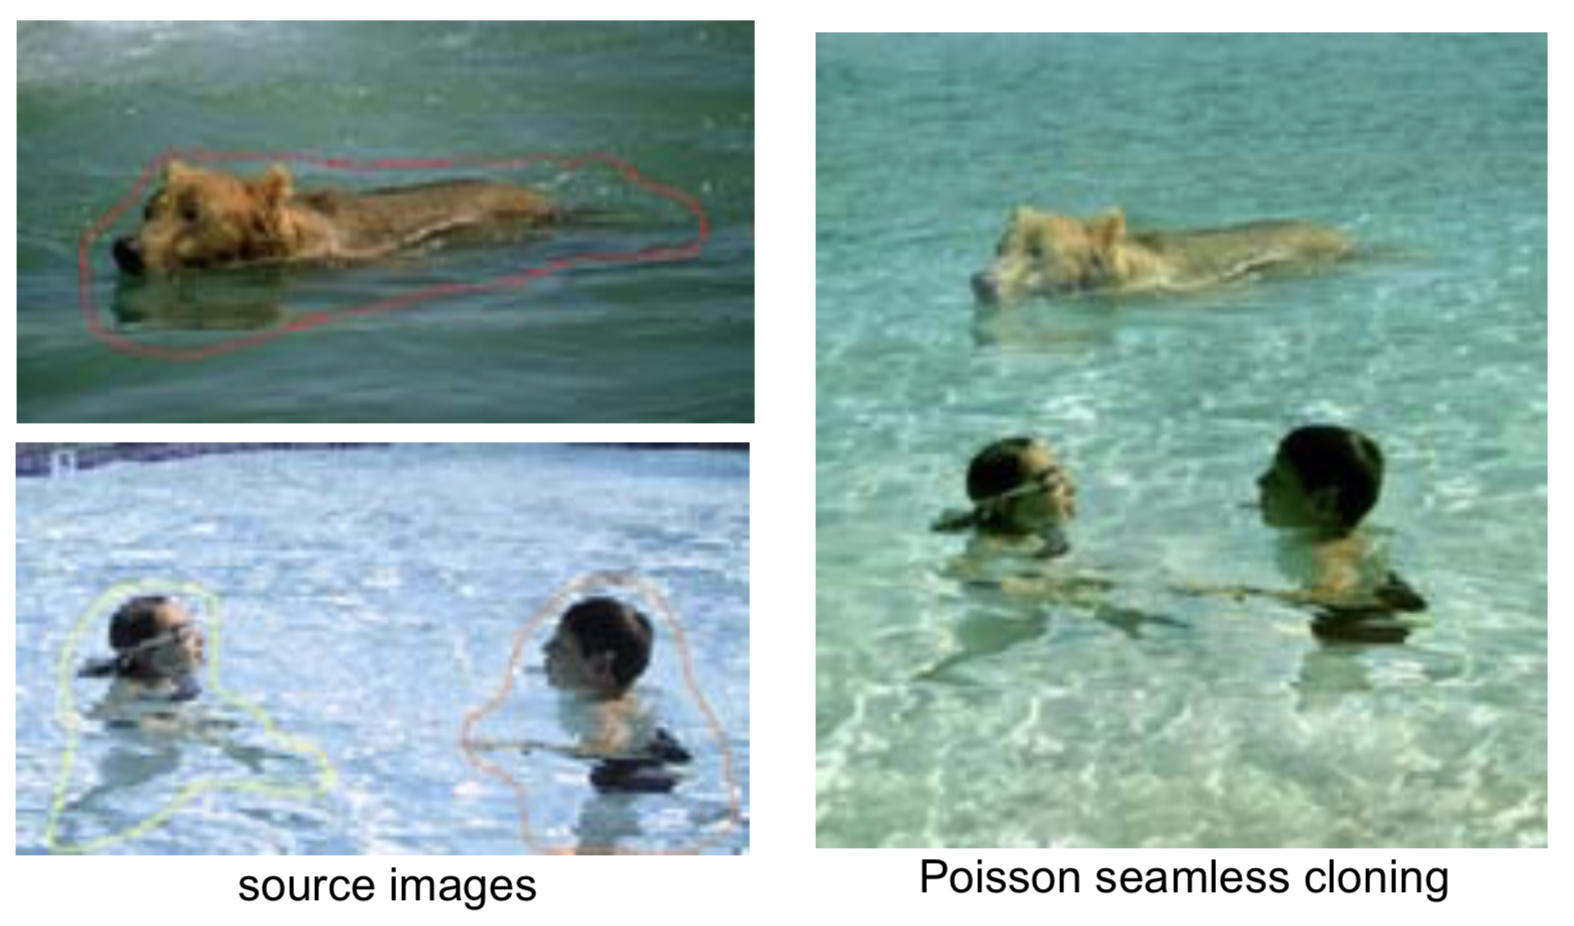
\includegraphics[width=3.8in]{resource/possion_cloning_2.png}        
    \end{figure}
\end{frame}

\begin{frame}
    \frametitle{How to Solve}
    \begin{itemize}
        \item Make the interior of $\Omega$ ``look like'' $S(x,y)$ 
        \item Also want the color to match between $S(x,y)$ and  $T(x,y)$        
    \end{itemize}    
\end{frame}

\begin{frame}
    \frametitle{How to Solve}
    \begin{itemize}
        \item Transfer the ``edges'' of the $S(x,y)$ to into $\Omega$
        \item Computer colors inside $\Omega$ as close as possible with pixels from $T(x,y)$ surrounding $\Omega$
        \item We want the gradient of the composite image, $\nabla I(x,y)$, inside $\Omega$ as close possible to $\nabla S(x,y)$
        \item Subject to the constraint the result must match existing values of $T(x,y)$ on the boundary $\partial \Omega$
    \end{itemize}    
\end{frame}

\begin{frame}
    \frametitle{How to solve}
    Miminize:
    \begin{equation} 
        \label{eq:1}
        \min_{I(x,y) \in \Omega} \iint \limits_{\Omega} ||\nabla I(x,y) - \nabla S(x,y) ||^{2}dxdy        
    \end{equation}
    Subject to:
    \begin{equation}
        \label{eq:2}
        I(x,y) = T(x,y), \quad (x,y) \in \partial \Omega        
    \end{equation}
\end{frame}

\begin{frame}
    \frametitle{Euler-Lagrange Equation}
    A fundamental equation of {\bf Calculus of Variations} states that, if $J$ is defined by an integral of the form:
    \[
        J= \int F(x,f, f_x)dx
    \]
    Then $J$ has a stationary value if the following differential equation is satisfied:
    \[
        \frac{\partial F}{\partial f} - \frac{d}{dx}\frac{\partial F}{\partial f_x}=0
    \]
\end{frame}

\begin{frame}
    \frametitle{Euler-Lagrange Equation}
    In our case, we have:
    \begin{equation}
        \label{eq:3}
        \begin{split}
            F(x,y) &= ||\nabla I(x,y) - \nabla S(x,y) ||^{2}  \\ 
                   &= \bigg(\frac{\partial I}{\partial x} - \frac{\partial S}{\partial x}\bigg)^2 
                     + \bigg(\frac{\partial I}{\partial y} - \frac{\partial S}{\partial y}\bigg)^2 
        \end{split}        
    \end{equation}
    $I(x,y)$ that solves Equation \ref{eq:1} is a solution of the {\bf Euler-Lagrange equation}:
    \begin{equation}
        \label{eq:4}
        \frac{\partial F}{\partial I}
        -\frac{d}{dx}\frac{\partial F}{\partial I_x}
        -\frac{d}{dy}\frac{\partial F}{\partial I_y}=0, 
        \quad (x,y) \in \Omega 
    \end{equation}
\end{frame} 


\begin{frame}
    \frametitle{Possion Equation}
    Plugging in Equation \ref{eq:3} into Equation \ref{eq:4}:
    \begin{equation}
        \label{eq:5}
        2\bigg(\frac{\partial^2 I}{\partial x^2}-\frac{\partial S^2}{\partial x^2}\bigg) 
        + 2\bigg(\frac{\partial^2 I}{\partial y^2}-\frac{\partial^2 S}{\partial y^2}\bigg)     
    \end{equation} 
    We have:   
    \begin{equation}
        \label{eq:6}
        \nabla^2 I(x,y) = \nabla^2 S(x,y), \quad (x,y) \in \Omega 
    \end{equation}    
    Where:
    \[
        \nabla^2I=\frac{\partial^2 I}{\partial x^2}+\frac{\partial^2 I}{\partial y^2}
    \]
    Subject to:   
    \begin{equation}
        \label{eq:7}
         I(x,y) = T(x,y), \quad (x,y) \in \partial\Omega 
    \end{equation}        
    Note, an equation of the form \ref{eq:6} is called a {\bf Possion equation}, and a constraint of the form of  Equation \ref{eq:7} is called a {\bf Dirichlet boundary condition}.
\end{frame} 

\begin{frame}
    \frametitle{Discrete Poisson solver}
    \begin{itemize}
        \item In Equation \ref{eq:6} the Laplacian of the new image $I(x,y)$ is equal to the Laplacian of the source image $S(x,y)$ inside $\Omega$. 
        \item More powerful to mim. the difference using a {\it guidance vector field} $\vec{{\bf S}}=(S_x(x,y), S_y(x,y))$ at every pixel $(x,y)$, Equation \ref{eq:6} change to:        
        \begin{equation}
            \label{eq:8}
            \nabla^2 I(x,y) = div
            \begin{bmatrix}
                S_x(x,y) \\[0.3em]
                S_y(x,y) \\[0.3em]                
            \end{bmatrix}
            = \frac{\partial S_x}{\partial x}+\frac{\partial S_y}{\partial y}, \quad (x,y) \in \Omega
        \end{equation} 
        \item Create discrete version of Equation \ref{eq:6} and \ref{eq:7} 
        \item Use 4 neighborhood operator to approximiate the Laplacian operator 
        \[
        \begin{bmatrix}
            0 & 1 & 0       \\[0.3em]
            1 & -4 & 1      \\[0.3em]
            0 & 1 & 0       \\[0.3em]
          \end{bmatrix}
        \]
    \end{itemize}        
\end{frame} 

\begin{frame}
    \frametitle{Discrete Poisson solver}
    \begin{itemize}    
        \item Each pixel $p=(x,y)$ in $\Omega$ generates a linear equation for unknown values in $I(x,y)$    
        \begin{item} 
            Two cases, for the 4-neighborhood $N(p)$: 
            \begin{figure}[!ht]
                \centering
                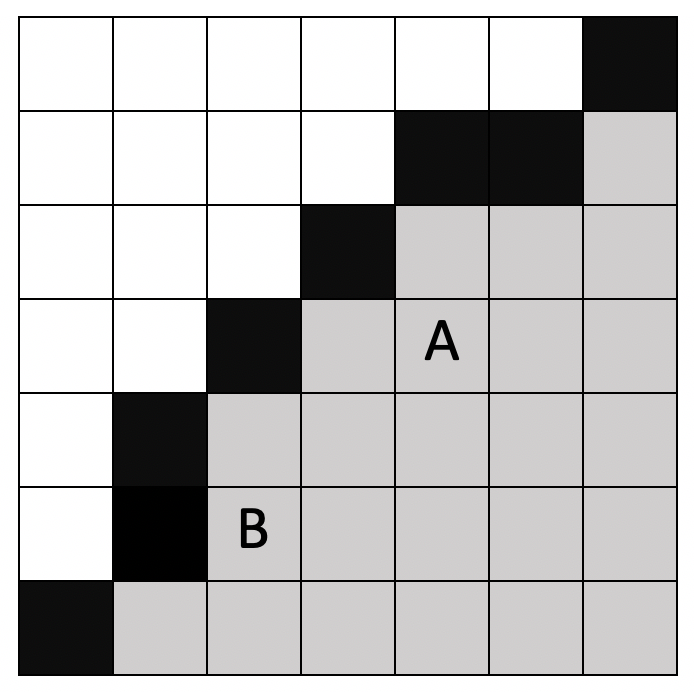
\includegraphics[width=2.2in]{resource/grid.png}            
            \end{figure}            
        \end{item}
    \end{itemize}
\end{frame} 

\begin{frame}
    \frametitle{Discrete Poisson solver}    
        \begin{enumerate}
            \item $N(p) \in \Omega$ The neighborhoods of $p$ are fully contained in $\Omega$ and the Laplacian: 
            $I(x+1,y)+I(x-1,y)+I(x,y+1)+I(x,y-1)-4I(x,y)=S(x+1,y)+S(x-1,y)+S(x,y+1)+S(x,y-1)-4S(x,y)$
            \item $N(p) \notin \Omega$ Not all neighborhoods of $p$ are contained in $\Omega$, at least one neighborhood is in $\partial \Omega$:
            \[
                \begin{split}
                    \Bigg(\sum_{q \in N(p) \cap \Omega}I(q)\Bigg)     
                    +\Bigg(\sum_{q \in N(p) \cap \partial \Omega}T(q)\Bigg)     
                    -4I(x,y) &= \\ S(x+1,y)+S(x-1,y)+S(x,y+1)+S(x,y-1)-4S(x,y)
                \end{split}
            \]
        \end{enumerate}    
\end{frame} 


\begin{frame}
    \frametitle{Discrete Poisson solver}    
    \begin{itemize}
        \item This reduces to the sparse linear systems:        
    \end{itemize}
    \[    
        \begin{pmatrix}
        1 & 1 & -4 & 1 &  1  & \cdots & \cdots & \cdots &  0\\
        0 & 1 & 1 & -4 & 1 & 1 & \cdots & \cdots & 0 \\
        0 & 0 & 1 & 1 & -4 & 1 & 1 & \cdots & 0 \\
        \vdots &  &  &  &  &  &  &  &  \vdots \\
        \vdots &  &  &  &  &  &  &  &  \vdots \\
        \vdots &  &  &  &  &  &  &  &  \vdots \\
        0 &  &  &  &  &  &  &  &  0 \\
        \vdots &  &  &  &  &  &  &  &  \vdots \\
        0 & \cdots & \cdots & \cdots & \cdots & \cdots & \cdots & \cdots & 1 \\
        \end{pmatrix}
        \begin{pmatrix}
            x_1 \\
            x_2 \\
            \vdots\\
            \vdots\\
            \vdots\\
            \vdots\\
            \vdots\\
            \vdots\\            
            x_n 
        \end{pmatrix} = 
        \begin{pmatrix}
            0 \\
            0 \\
            b_1\\
            b_2\\
            0 \\
            \vdots\\
            b_3\\
            \vdots\\            
            \vdots\\            
            b_n 
        \end{pmatrix}
    \]
\end{frame} 


% %===================== extra stuff we don't really care ========================









































% \begin{frame}
% \frametitle{Blocks of Highlighted Text}
% \begin{block}{Block 1}
% Lorem ipsum dolor sit amet, consectetur adipiscing elit. Integer 


% lectus nisl, ultricies in feugiat rutrum, porttitor sit amet augue. Aliquam ut tortor mauris. Sed volutpat ante purus, quis accumsan dolor.
% \end{block}

% \begin{block}{Block 2}
% Pellentesque sed tellus purus. Class aptent taciti sociosqu ad litora torquent per conubia nostra, per inceptos himenaeos. Vestibulum quis magna at risus dictum tempor eu vitae velit.
% \end{block}

% \begin{block}{Block 3}
% Suspendisse tincidunt sagittis gravida. Curabitur condimentum, enim sed venenatis rutrum, ipsum neque consectetur orci, sed blandit justo nisi ac lacus.
% \end{block}
% \end{frame}

% %------------------------------------------------

% \begin{frame}
% \frametitle{Multiple Columns}
% \begin{columns}[c] % The "c" option specifies centered vertical alignment while the "t" option is used for top vertical alignment

% \column{.45\textwidth} % Left column and width
% \textbf{Heading}
% \begin{enumerate}
% \item Statement
% \item Explanation
% \item Example
% \end{enumerate}

% \column{.5\textwidth} % Right column and width
% Lorem ipsum dolor sit amet, consectetur adipiscing elit. Integer lectus nisl, ultricies in feugiat rutrum, porttitor sit amet augue. Aliquam ut tortor mauris. Sed volutpat ante purus, quis accumsan dolor.

% \end{columns}
% \end{frame}

% %------------------------------------------------
% \section{Second Section}
% %------------------------------------------------

% \begin{frame}
% \frametitle{Table}
% \begin{table}
% \begin{tabular}{l l l}
% \toprule
% \textbf{Treatments} & \textbf{Response 1} & \textbf{Response 2}\\
% \midrule
% Treatment 1 & 0.0003262 & 0.562 \\
% Treatment 2 & 0.0015681 & 0.910 \\
% Treatment 3 & 0.0009271 & 0.296 \\
% \bottomrule
% \end{tabular}
% \caption{Table caption}
% \end{table}
% \end{frame}

% %------------------------------------------------

% \begin{frame}
% \frametitle{Theorem}
% \begin{theorem}[Mass--energy equivalence]
% $E = mc^2$
% \end{theorem}
% \end{frame}

% %------------------------------------------------

% \begin{frame}[fragile] % Need to use the fragile option when verbatim is used in the slide
% \frametitle{Verbatim}
% \begin{example}[Theorem Slide Code]
% \begin{verbatim}
% \begin{frame}
% \frametitle{Theorem}
% \begin{theorem}[Mass--energy equivalence]
% $E = mc^2$
% \end{theorem}
% \end{frame}\end{verbatim}
% \end{example}
% \end{frame}

% %------------------------------------------------

% \begin{frame}
% \frametitle{Figure}
% Uncomment the code on this slide to i nclude your own image from the same directory as the template .TeX file.
% %\begin{figure}
% %\includegraphics[width=0.8\linewidth]{test}
% %\end{figure}
% \end{frame} 

% %------------------------------------------------

% \begin{frame}[fragile] % Need to use the fragile option when verbatim is used in the slide
% \frametitle{Citation}
% An example of the \verb|\cite| command to cite within the presentation:\\~

% This statement requires citation \cite{p1}.
% \end{frame}

% %------------------------------------------------

\begin{frame}
\frametitle{References}
\footnotesize{
\begin{thebibliography}{99} % Beamer does not support BibTeX so references must be inserted manually as below
\bibitem[Smith, 2012]{p1} John Smith (2012)
\newblock Title of the publication
\newblock \emph{Journal Name} 12(3), 45 -- 678.
\end{thebibliography}
}
\end{frame}

%------------------------------------------------

\begin{frame}
\Huge{\centerline{The End}}
\end{frame}

%----------------------------------------------------------------------------------------

\end{document} 